\documentclass{article}

\usepackage[utf8]{inputenc}
\usepackage[ngerman]{babel}
\usepackage{amsmath}
\usepackage{url}
\usepackage[pdftex]{graphicx}
\usepackage{listings}
 
\title{Object Caching\\Project Proposal}
\author{Lukas Hofmaier, Raphael Kohler, Timon Brüllmann}
\date{\today}
\begin{document}
\maketitle
\section{Betreuer}
J.M.Joller  Abteilung für Informatik HSR/FHO

\section{Motivation}
Das Datenverarbeitungssystem Mercury ermöglicht es Clients Methoden von Objekten über das Netzwerk aufzurufen. Dabei entstehen unter anderem folgende zwei Problembereiche, auf welche das Augenmerk dieser Studienarbeit gelegt wird:

\begin{itemize}
\item Clients können Werte von Instanzvariablen von Objekten auf dem Server lesen. Die Clients können diese Werte im Hauptspeicher abspeichern und zu einem späteren Zeitpunkt in einer kausal abhängigen Methode als Argument einsetzen. Dabei kann ein "Lost Update" auftreten.
\item Alle Methodenaufrufe werden über das Netzwerk an den Server gesendet. Die Methodenaufrufe auf den Clients sollen schneller werden.
\end{itemize}

\section{Ziele der Arbeit}

\subsection{Prioritaeten}
\label{sec:prioritaeten}

\begin{enumerate}
\item Das "Lost Update"-Problem soll vermieden werden.
\item Die Abhandlung der Schreib -und Lesezugriffe auf das Objekt, welches auf dem Server liegt, soll für den Client möglichst schnell passieren.
\end{enumerate}

\subsection{Hauptziele}
\label{sec:hauptziele}

\subsubsection{RMI mit Concurrency Control}
\label{sec:rmi-mit-concurrency}

In dieser Semesterarbeit soll nun ein Konzept erarbeitet werden, welches Lost Updates bei kausal abhängigen Methoden verhindert.  Es soll ein vereinfachtes RMI System implementiert werden. Dieses System soll zeigen, ob sich das Konzept einfach realisieren lässt.

\subsubsection{Testframework}
\label{sec:testframework}

Um das System zu testen, wird parallel dazu ein Testframework entwickelt. Dieses Framework soll in der Lage sein, unterschiedliche RMI System als Server und Client zu starten. Das Testframework ist in der Lage, eine Szenariobeschreibung einzulesen und dieses Szenario mit dem zu testenden System durchzuspielen. Ein Szenario besteht aus einer Abfolge von Methoden-Aufrufen, welche der jeweilige Client tätigen muss. Das Framework sammelt dabei Messdaten über die Zeitdauer der einzelnen Methodenaufrufe. Die Messdaten sollen es ermöglichen abzuwägen, welche Systeme mit welchen Parameter sich für welchen Anwendungszweck eignen.
Weiter registriert das Testframework das Auftreten von Schreib-Konfikten bei Aufruf von Schreibmethoden.

\subsection{Erweiterte Ziele}
\label{sec:erweiterte-ziele}

\subsubsection{Object Caching}
\label{sec:object-caching}

Um die Dauer von Methodenaufrufen zu verkürzen, soll das RMI System um einen Object Cache erweitert werden. Methoden ohne Seiteneffekte werden auf den Objekten im Cache ausgeführt. Für das System wird ein passendes Konsistenzmodell ausgewählt. Dieses Modell wird durch ein geeignetes Konsistenzprotokoll durchgesetzt. Die Unterscheidung von Lese und Schreib- Methoden muss durch den User gemacht werden.

\subsubsection{Entwicklung neuer Szenarien}
\label{sec:entwicklung-neuer-szenarien}

Um die Lösungen mit und ohne Cache miteinander vergleichen zu können, müssen neue Testszenarien geschrieben werden.

\subsubsection{Feingranulares Locking}
\label{sec:feingr-lock}

Der Concurrency-Mechanismus soll es ermöglichen, dass Anfragen parallel ausgeführt werden können.

\subsection{Szenarien}
\label{sec:szenario}

Als Ausgangslage für das gesamte Projekt wird folgendes Szenario eingesetzt:

\subsubsection{Deployement}
\label{sec:deployement}

Es wird ein verteiltes System mit einem Server und zwei Clients verwendet.
\begin{center}
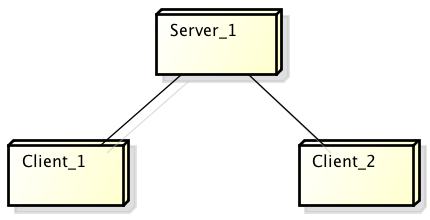
\includegraphics[scale=0.85]{Deployment.png}
\end{center}

\subsubsection{Kausaler Zusammenhang}
\label{sec:kaus-zusamm}

Die Clients möchten den Kontostand um 10 \% erhöhen. Sie führen dazu folgende Schritte aus
\begin{lstlisting}
b = getBalance();
setBalance( b * 1.1 );
\end{lstlisting}
Diese Schritte werden zum Prozess ‘‘Kontostand Erhöhen’’ zusammengefasst.

\subsubsection{Account Typ}
\label{sec:account-typ}

Auf einem Server wird ein Account-Objekt instanziert.
Das Interface von Account sieht wie folgt aus:
\begin{lstlisting}
public interface Account {
    public int getBalance();
    public void setBalance(int balance);    
}
\end{lstlisting}
Zwischen getBalance und setBalance besteht ein kausaler Zusammenhang. setBalance darf nur ausgeführt werden, wenn das Argument balance aktuell ist. Ist der Wert nicht mehr aktuell, wird der "Kontostand-Erhöhen"-Prozess abgebrochen. Der Client wiederholt in diesem Fall den gesamten Prozess (aktuelle Daten holen, Daten schreiben) noch automatisch.

Dem Client ist das Interface Account bekannt. Das Interface wird vor Prozessstart deployed.
Zwei Client beschaffen sich eine Referenz in Form eines Proxy-Objektes auf das Account-Objekt. 

\subsubsection{TestFramework}
\label{sec:testframework-1}


Bei jedem Szenario werden folgende Messdaten festgehalten.
\begin{itemize}
\item durchschnittliche Dauer des Methodenaufrufs getBalance()
\item durchschnittliche Dauer des Methodenaufrufs setBalance()
\item Anzahl aufgetretene Konflikte
\item Dauer eines setBalance(); Methodenaufrufs bei Konfliktsituation
  \begin{itemize}
  \item Zeitdifferenz zwischen erstem setBalance bis erfolgreichem setBalance
  \item Zeitdifferenz zwischen setBalance und Empfang der zugehörigen Exception
  \end{itemize}
\end{itemize}

\subsubsection{Konfliktloser Zugriff}
\label{sec:konfl-zugr}

Das Szenario soll zeigen wie lange Methodenaufrufe dauern, wenn keine Konflikte auftreten. Ein Client führt den Prozess Kontostand-Erhöhen 10000-mal aus.

\subsubsection{Race Condition}
\label{sec:race-condition}
Das Szenario soll zeigen wie viele Konflikte auftreten, wenn beide Clients permanent Kontoerhöhungen ausführen wollen.
Beide Clients führen den Prozess Kontostand-Erhöhen 10000 mal aus. Server startet die Clients hintereinander mit einer möglichst kleinen Zeitdifferenz.

\subsubsection{Erzwungene Konflikte}
\label{sec:erzwungene-konflikte}

In diesem Szenario soll jeder setBalance-Aufruf von Client 2 zu einer Konfliktsituation führen. Damit sind Konfliktsituation nicht dem Zufall überlassen, sondern treten zuverlässig auf und können besser analysiert werden.

Client 1 führt ununterbrochen Kontoerhöhungen aus. Client 2 führt 100 Kontoerhöhungen aus. Client 2 wartet nach dem getBalance()-Aufruf 10ms. In dieser Zeit sollte Client1 eine Schreiboperation ausführen und die Daten im Speicher von Client 2 werden veraltet.

\section{Durchführung}
Mit dem Betreuer dieser Arbeit findet eine wöchentliche Sitzung statt. Dabei werden die Fortschritte besprochen und falls vorhanden offene Fragen diskutiert. Die Länge der Sitzung ist daher variabel, je nachdem ob und wieviele offene Fragen und Probleme bestehen.


\vspace{1cm}

\noindent Rapperswil, den\\
Der verantwortliche Dozent\\
\end{document}